%%%%%%%%%%%%%%%%%%%%%%%%%%%%%%%%%%%%%%%%%%%%%%%%%%%%%%%%%%%%%%%%%%%%%%%%%%%%%%%%%%
\begin{frame}[fragile]\frametitle{}
\begin{center}
{\Large Applications to Mechanical Engineering}
\end{center}
\end{frame}

%%%%%%%%%%%%%%%%%%%%%%%%%%%%%%%%%%%%%%%%%%%%%%%%%%%%%%%%%%%
\begin{frame}[fragile]\frametitle{The Announcement}
\begin{center}
{\Large ``Revitalizing manufacturing through AI''}
\end{center}
\begin{itemize}
\item  AI is already transforming the IT industry.
\item It is now time to for an AI-powered society.
\item We will initially focus on the manufacturing industry.
\end{itemize}

\tiny{(Reference: ``Medium'' - Andrew Ng, Dec 14,2017)}
\end{frame}

%%%%%%%%%%%%%%%%%%%%%%%%%%%%%%%%%%%%%%%%%%%%%%%%%%%%%%%%%%%
\begin{frame}[fragile]\frametitle{Why Manufacturing?}
\begin{itemize}
\item  Manufacturing touches every part of society.
\item Need to help not just bits and pixels but physical world.
\end{itemize}

\end{frame}

%%%%%%%%%%%%%%%%%%%%%%%%%%%%%%%%%%%%%%%%%%%%%%%%%%%%%%%%%%%
\begin{frame}[fragile]\frametitle{Challenges facing manufacturing}
\begin{itemize}
\item  Variable quality and yield, 
\item Inflexible production line design
\item Inability to manage capacity
\item and rising production costs.
\end{itemize}
ML to help address them.
\end{frame}

%%%%%%%%%%%%%%%%%%%%%%%%%%%%%%%%%%%%%%%%%%%%%%%%%%%%%%%%%%%
\begin{frame}[fragile]\frametitle{Challenges facing manufacturing}
More help in
\begin{itemize}
\item  Shorten design cycles, 
\item Remove supply-chain bottlenecks, 
\item Reduce materials and energy waste, 
\item and improve production yields.
\end{itemize}

\end{frame}


%%%%%%%%%%%%%%%%%%%%%%%%%%%%%%%%%%%%%%%%%%%%%%%%%%%%%%%%%%%
\begin{frame}[fragile]\frametitle{Why now?}
\begin{center}
{\Large ``Industry today is experiencing a never seen increase in available data'' }
\end{center}
Sources:
\begin{itemize}
\item  Environmental data
\item Sensor data from production line
\item Machine tool parameters
\item Logistics, transaction data
\item Customer demand data.
\end{itemize}
\tiny{(Reference: What is smart manufacturing? Time Magazine - Chand \& Davis, 2010)}
\end{frame}

%%%%%%%%%%%%%%%%%%%%%%%%%%%%%%%%%%%%%%%%%%%%%%%%%%%%%%%%%%%
\begin{frame}[fragile]\frametitle{How ML can help?}

\begin{itemize}
\item  Ability to handle high-dimensional problems
\item SVM handling high dimensionality ($>1000$) very well. 
\item Concerns: Over-fitting
\end{itemize}
{\tiny (Ref: ``Machine learning in manufacturing: advantages, challenges, and applications''- Thorsten Wuest, et al)}
\end{frame}


%%%%%%%%%%%%%%%%%%%%%%%%%%%%%%%%%%%%%%%%%%%%%%%%%%%%%%%%%%%
\begin{frame}[fragile]\frametitle{How ML can help?}

\begin{itemize}
\item  Ability to reduce complexity
\item Present transparent and concrete advice for practitioners 
\item E.g. monitor XX and parameter YY at checkpoint ZZ
\item ML finds important features, thresholds
\end{itemize}
{\tiny (Ref: ``Machine learning in manufacturing: advantages, challenges, and applications''- Thorsten Wuest, et al)}
\end{frame}

%%%%%%%%%%%%%%%%%%%%%%%%%%%%%%%%%%%%%%%%%%%%%%%%%%%%%%%%%%%
\begin{frame}[fragile]\frametitle{How ML can help?}

\begin{itemize}
\item  Ability to adapt to changing environment
\item New data, new training, new model.
\end{itemize}
{\tiny (Ref: ``Machine learning in manufacturing: advantages, challenges, and applications''- Thorsten Wuest, et al)}
\end{frame}

%%%%%%%%%%%%%%%%%%%%%%%%%%%%%%%%%%%%%%%%%%%%%%%%%%%%%%%%%%%
\begin{frame}[fragile]\frametitle{New wave: IoT}
``Internet of Things''
\begin{itemize}
\item  IOT is connecting things to the Internet
\item Not the same as connecting things to the cellular network! 
\item IOT personal (Health apps) 
\item IOT Machine (Machine 2 Machine M2M) 
\item IoT Everywhere (5G, wifi)
\end{itemize}
\end{frame}

%%%%%%%%%%%%%%%%%%%%%%%%%%%%%%%%%%%%%%%%%%%%%%%%%%%%%%%%%%%
\begin{frame}[fragile]\frametitle{New wave: IoT}
IoT Data
\begin{itemize}
\item Sensors everywhere.
\item By 2020,50 billion connected devices.
\item Wearables, cars, machines, cities.
\end{itemize}
\end{frame}

%%%%%%%%%%%%%%%%%%%%%%%%%%%%%%%%%%%%%%%%%%%%%%%%%%%%%%%%%%%
\begin{frame}[fragile]\frametitle{New wave: IoT}
IoT and Machine Learning
\begin{itemize}
\item Basic idea of machine learning is to build a mathematical model based on training data(learning stage) ,  predict results for new data(prediction stage) and tweak the model based on new conditions
\item  IoT creates a lot of contextual data 
\item Use the scale of IoT data to gain new insights
\end{itemize}
\end{frame}

%%%%%%%%%%%%%%%%%%%%%%%%%%%%%%%%%%%%%%%%%%%%%%%%%%%%%%%%%%%
\begin{frame}[fragile]\frametitle{New wave: IoT}
IoT ML Applications
\begin{itemize}
\item  Consumer : bio sensors(real time tracking)
\item  Enterprise : Complex machinery (preventative maintenance), asset efficiency.
\item Public infrastructure: Smart Cities, Dynamically adjust traffic lights
\end{itemize}
\end{frame}
%%%%%%%%%%%%%%%%%%%%%%%%%%%%%%%%%%%%%%%%%%%%%%%%%%%%%%%%%%%
\begin{frame}[fragile]\frametitle{Sample Applications: Tool Wear Estimation}
 Hidden Markov Model
\begin{center}
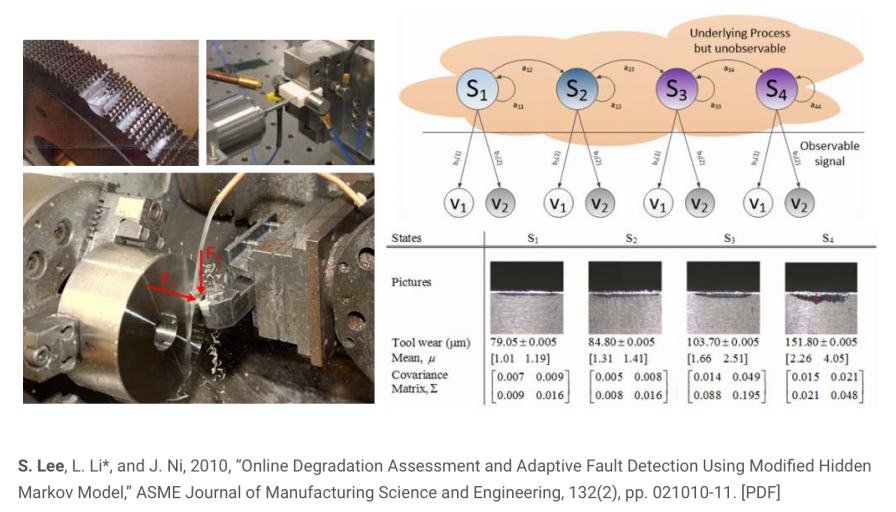
\includegraphics[width=0.8\linewidth,keepaspectratio]{mechapp2}
\end{center}
\end{frame}



% %%%%%%%%%%%%%%%%%%%%%%%%%%%%%%%%%%%%%%%%%%%%%%%%%%%%%%%%%%%
% \begin{frame}[fragile]\frametitle{Other Applications: Robot  Playing Piano}

% \begin{center}
% 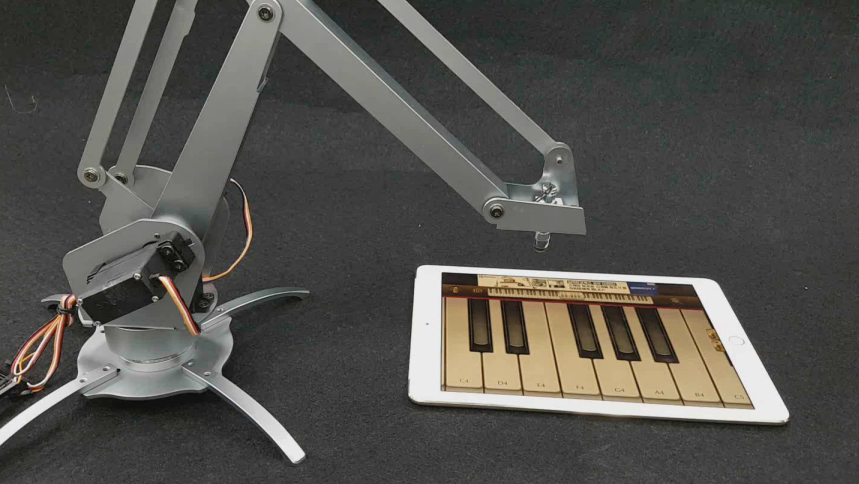
\includegraphics[width=0.8\linewidth,keepaspectratio]{mechapp1}
% \end{center}
% {\tiny (Ref: Machine Learning and Deep Learning in Manufacturing - Prof. Seungchul Lee)}
% \end{frame}

%%%%%%%%%%%%%%%%%%%%%%%%%%%%%%%%%%%%%%%%%%%%%%%%%%%%%%%%%%%
\begin{frame}[fragile]\frametitle{Ideas for new applications}
Project ideas?
\begin{itemize}
\item Kaggle: https://www.kaggle.com/datasets
\item UCI: http://archive.ics.uci.edu/ml/index.php
\item  Other: http://deeplearning.net/datasets/
\end{itemize}
\end{frame}






%%%%%%%%%%%%%%%%%%%%%%%%%%%%%%%%%%%%%%%%%%%%%%%%%%%%%%%%%%%%
%\begin{frame}[fragile]\frametitle{Some types of algorithms}
%\begin{itemize}
%\item Prediction: predicting a variable from data
%\item Classification: assigning records to predefined groups
%\item Clustering: splitting records into groups based on similarity
%\item Association learning: seeing what often appears together
%\end{itemize}
%
%\end{frame}
%
%
%
%%%%%%%%%%%%%%%%%%%%%%%%%%%%%%%%%%%%%%%%%%%%%%%%%%%%%%%%%%%%
%\begin{frame}[fragile]\frametitle{How to figure out? A dumb way}
%Step 1: Start with each weight set to 1.0:
%\begin{lstlisting}
%def estimate_house_sales_price(num_of_bedrooms, sqft, neighborhood):
%	price = 0
%	price += num_of_bedrooms * 1.0
%	price += sqft * 1.0
%	price += neighborhood * 1.0
%	price += 1.0
%
% return price
%\end{lstlisting}
%\end{frame}
%


